\documentclass{article}
\usepackage[T1]{fontenc}
\usepackage[utf8]{inputenc}
\usepackage{amsmath,amssymb,amsfonts}
\usepackage[english,main=russian]{babel}
\usepackage{graphicx}
\graphicspath{{.}}

\begin{document}

\noindent \textbf{1. В результате медицинского обследования один из тестов выявил у человека серьезное заболевание. Данный тест имеет высокую точность 99\% (вероятность позитивного ответа при наличии заболевания 99\%, вероятность отрицательного ответа при отсутствии заболевания также 99\%). Однако, выявленное заболевания является достаточно редким и встречается только у одного человека на 10000. Вычислить вероятность того, что у обследуемого человека действительно есть выявленное заболевание.}

$P(M) = 0.0001$ - вероятность быть больным. $P(T|M) = 0.99$ -  вероятность того, что тест показал $"$человек болен$"$ при условии, что человек болен. Тогда $P(T|\overline M) = 1 - P(T|M) = 0.01$ - вероятность того, что тест показал $"$человек болен$"$ при условии, что человек неболен. Найдем вероятность того, что тест покажет $"$человек болен$"$ - это может случиться, если человек действительно болен и тест не соврал или если человек неболен, но тест показал неправильный результат, получаем: $P(T) = P(M)P(T|M)+P(\overline M)P(T|\overline M) = 0.0001 * 0.99 + 0.9999 * 0.01 = 0.010098$. Тогда вероятность того, что человек болеет при условии, что тест показал $"$человек болен$"$ равна (по формуле Байеса): $P(M|T) = \frac{P(M)P(T|M)}{P(T)} = \frac{0.0001*0.99}{0.010098} = \frac{1}{102} \approx 0.0098$.

\vspace{2mm}

\noindent \textbf{2. Показать, что $P(A|B)=P(A|BC)P(C|B)+P(A|B\overline C)P(\overline C|B).$}

\vspace{3mm}

Будем считать, что $0 < P(B) < 1 \land 0 < P(C) < 1$, чтобы нигде не возникло деление на 0.

Рассмотрим $P(A|BC)P(C|B) = P(A|BC)\frac{P(CB)}{P(B)} = \frac{P(A|BC)P(BC)}{P(B)} = \frac{P(ABC)}{P(B)}$
\vspace{1mm}

 и $P(A|B\overline C)P(\overline C|B) = P(A|B\overline C)\frac{P(\overline C B)}{P(B)} = \frac{P(A|B\overline C)P(B\overline C)}{P(B)} = \frac{P(AB\overline C)}{P(B)}$. 
\vspace{1mm}

Тогда $P(A|BC)P(C|B)+P(A|B\overline C)P(\overline C|B) = \frac{P(ABC)}{P(B)} + \frac{P(AB\overline C)}{P(B)} =$
\vspace{1mm}

$= \frac{P(ABC)+P(AB\overline C)}{P(B)} = [P - \text{аддитивная функция}] = \frac{P(ABC\cup AB\overline C)}{P(B)} =$

$ = \frac{P(AB(C\cup \overline C))}{P(B)} = \frac{P(AB)}{P(B)} = P(A|B)$. Ч.т.д. 
\vspace{2mm}

\noindent \textbf{3. Дано натуральное число $4\leq n \leq 48$. Из тщательно перемешанной колоды в 52 карты одновременно были взяты $n$ карт. На одну из этих $n$ карт посмотрели, она оказалась тузом. После этого она возвращается в набор взятых карт и эти $n$ карт перемешиваются. После этого из них выбирается одна карта и открывается. Найдите вероятность того, что открытая карта является тузом.}

Примем во внимание то, что в колоде все тузы различны. Пусть $P(T)$ - вероятность того, что открытая карта является тузом. $P(T) = P(T_E) + P(T_N\overline T_E)$, где $P(T_E) = \frac{1}{n}$ - вероятность того, что снова открытая карта - тот же туз, что и был вытянут на предыдущем шаге, $P(T_N\overline T_E)$ - вероятность того, что окрытая карта - туз, но пока неизвестный.

Какая вероятность того, что в подколоде есть ещё один туз, кроме известного? Для любой карты одинаковая вероятность попасть в подколоду, всего тузов в исходной колоде 4, но один уже точно попал, поэтому вероятность того, что в подколоде есть ещё хотя бы один туз, равна $\frac{3}{51} = \frac{1}{17}$. 

\vspace{1mm}

Можем найти $P(T_N \overline T_E) = P(T_N|\overline T_E) P(\overline T_E)$, $P(T_N|\overline T_E) = \frac{1}{17}$ - вероятность того, что выпадет туз при условии, что не выпадет уже известный туз. Тогда  $P(T_N \overline T_E) = P(T_N|\overline T_E) P(\overline T_E) = \frac{1}{17} *(1 - \frac{1}{n})$.

\vspace{1mm}

Ответ: $P(T) = \frac{1}{n} + \frac{1}{17}*(1-\frac{1}{n})$.
\vspace{2mm}

\noindent \textbf{4. В семье есть 2 ребенка. Пол каждого ребенка — равновероятен. Какова вероятность того, что в семье есть девочка, если
\begin{itemize}
\item В семье точно есть один мальчик
\item В семье есть мальчик, который родился во Вторник.
\end{itemize}
    P.S. Вероятность родиться мальчиком или девочкой равны, выроятность родиться в любой из дней недели - равновероятно.}

Рассмотрим случай, когда в семье есть один мальчик. Тогда вероятность события, что в семье есть 2 девочки, является невозможной. И вероятность того, что в семье есть девочка, равна $\frac{2}{3}$, т.к. существуют только такие возможные события: в семье есть 2 мальчика, в семье есть девочка и мальчик, в семье есть мальчик и девочка - порядок детей имеет значение, он показывает, какого пола ребенок родился первее.

Ответ на первый пункт: $\frac{2}{3}$.

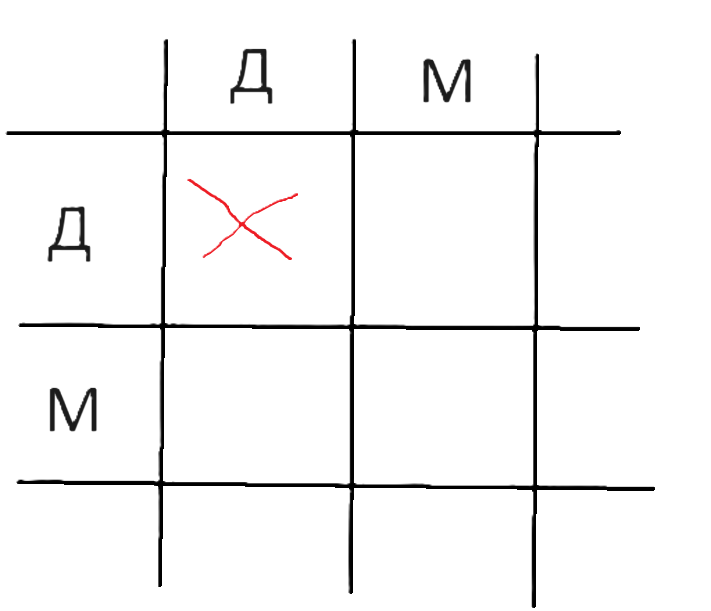
\includegraphics[width=30mm]{BoysAndGirls}

Теперь рассмотрим случай, когда в семье есть мальчик, родившийся во вторник. $P(D|M_2) = \frac{P(M_2|D)P(D)}{P(M_2)}$, где $P(D)$ - вероятность родиться девочке, $P(M_2)$ - вероятность родиться мальчику во вторник. В данном пункте имеется $14^2$ различных пар детей в семье: первый ребенок - мальчик или девочка, родившийся в один из 7 дней недели, второй - аналогично. 

Вероятность родиться девочке осталась такой же $P(D)= \frac{3}{4}$; $P(M_2) =$ $=\frac{27}{14^2}$ - т.к. для пары $(M_2,M_2)$ нет симметричной. $P(M_2|D) = \frac{14}{3*49}$ - т.к. общее число пар $(M_2,D_i) \lor (D_i, M_2)$, $\forall i = \overline{1..7}$ равно 14, а общее число пар, где есть девочка - $\frac{3}{4}14^2 = 3*49$.

\vspace{1mm}

Ответ: $P(D|M_2) = \frac{\frac{14}{3*49}*\frac{3}{4}}{\frac{27}{14^2}} = \frac{14}{27}$.

\vspace{2mm}

\noindent \textbf{5. В суде рассматривает дело об убийстве жены О. Джей Симпсона. Прокурор указал, что О. Джей Симпсон уже бил жену в прошлом. Адвокат ответил: "Убивают только одну из 2500 женщин, подвергающихся семейному насилию, так что это вообще нерелевантно". Суд согласился с адвокатом, верно ли это рассуждение?}

Такое рассуждение неверно, потому что адвокат не предоставил достаточный объем данных. Он утверждает, что $P(A|B)= \frac{1}{2500}$ - вероятность убийства женщины P(A) при условии, что она была подвергнута домашнему насилию P(B). Но по формуле полной вероятности $P(A) = P(A|B)P(B) + P(A|\overline B)P(\overline B)$, поэтому необходимо знать, как минимум, с какой вероятностью может произойти убийство женщины, которая не подвергалась домашнему насилию.

Вообще трудно не принимать во внимание такой факт, как домашнее насилие: статистика, которую предоставил адвокат, вряд ли отражает действительную ситуацию, потому что неописано как она собиралась, ведь не во всех случаях убийства можно точно установить, был подвержен человек домашнему насилию или нет; сам факт домашнего насилия говорит об агрессивном характере подозреваемого.

\end{document}